%
% Simple asymmetric two-column CV 
% Author: Sofia JIJON
%

\documentclass[a4paper,10pt]{article}
\usepackage[vmargin=1.5cm, hmargin=1.5cm]{geometry}
% !TEX root = Simple-CV.tex
%-------------------------------------------------------------------------------------------------------
% Packages
%-------------------------------------------------------------------------------------------------------
\usepackage[latin1]{inputenc}
\usepackage[T1]{fontenc}
\usepackage[english]{babel}
\usepackage{fontawesome}
\usepackage{datetime}
\usepackage[usenames,dvipsnames]{xcolor}
\usepackage[colorlinks=true, urlcolor=ColorTwo]{hyperref}
\usepackage{tikz}
\usepackage{hyperref}
\usepackage{setspace}
\usepackage{graphicx}
\usepackage{enumitem}
\usepackage{sectsty}
\usepackage{multicol}
\usepackage{adjustbox}
%-------------------------------------------------------------------------------------------------------
% Layout
%-------------------------------------------------------------------------------------------------------
\pagenumbering{gobble}
\renewcommand{\baselinestretch}{1.5} 
\setlength{\parindent}{0pt}

%
% Color theme
%
\definecolor{ColorOne}{RGB}{0,110,140} 	% Blue
\definecolor{ColorTwo}{RGB}{120,0,120} 	% Mauve
%\definecolor{ColorTwo}{RGB}{140,100,0} 	% Gold

\sectionfont{\color{ColorOne}} 
\subsectionfont{\color{ColorOne}} 

%
% Vertical line
%
\newcommand{\MyVerticalRule}{%
	\textcolor{ColorOne}{\rule{1pt}{\textheight}}
}

%
% Update
%
\newcommand{\LastUpdate}{%
\vfill
\centering \small
\textcolor{ColorOne}{Last updated: \monthname,~\the\year.}
}

%
% Skip
%
\newcommand{\MySkip}{
\vskip12pt
}

%
% Format hyperrefs
%
\newcommand{\myhref}[2]{%
\href{#1}{\textcolor{ColorTwo}{#2}}
}
%
% Format skill bullets
%
\newcommand{\SkillBull}[1]{%
\textcolor{ColorTwo}{#1}
}


%-------------------------------------------------------------------------------------------------------

\begin{document}
\thispagestyle{empty}

%-------------------------------------------------------------------------------------------------------
% Left column
%-------------------------------------------------------------------------------------------------------
\begin{adjustbox}{valign=t}
\begin{minipage}{0.3\textwidth} % Adapt width to your convenience
%----------------------------------------------------
% Please add a photo in 1x1 format
\begin{center}
\begin{tikzpicture}
	\clip (0,0) circle (2cm) node {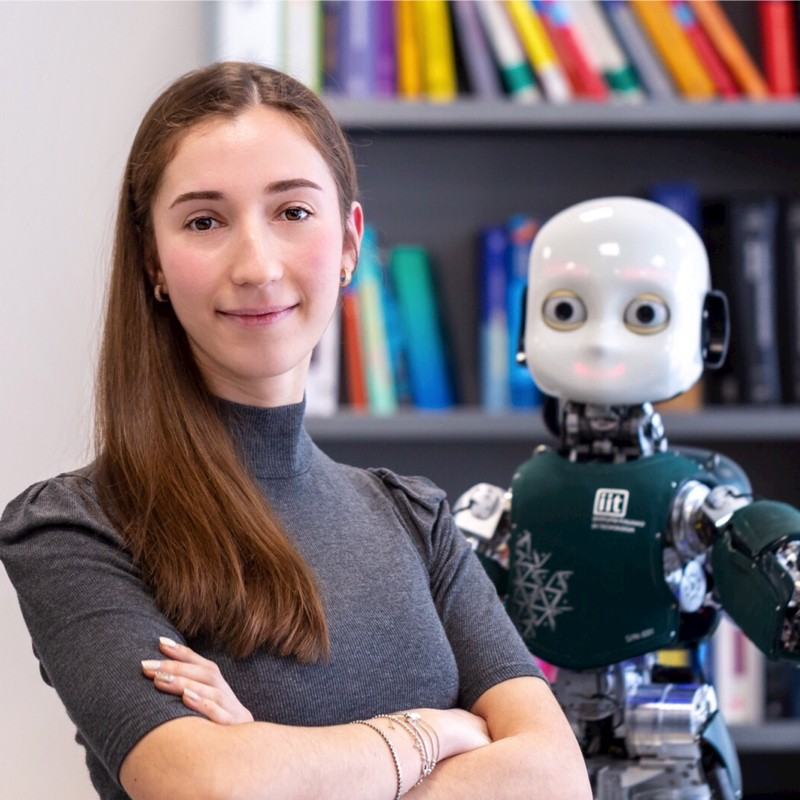
\includegraphics[width=4cm]{MyPhoto}};
\end{tikzpicture}

\MySkip 	% See MySetup.tex file

%----------------------------------------------------
{\LARGE \bfseries Ilaria Carlini}

\MySkip 	% See MySetup.tex file

Nationality: Italian\\
Date of birth: 07.01.1993

\MySkip 	% See MySetup.tex file

\textcolor{ColorTwo}{\faEnvelopeO} 
\myhref{mailto:ilariacarlini@icloud.com}{ilariacarlini@icloud.com} \\

\textcolor{ColorTwo}{\faGithub} 
\myhref{https://github.com/ilaria-carlini}{ilaria-carlini}

\textcolor{ColorTwo}{\faLinkedin} 
\myhref{https://www.linkedin.com/in/ilaria-carlini/}{ilaria-carlini}
\end{center}

\vfill

%----------------------------------------------------
\section*{Profile}
Dedicated and creative Full Stack Developer with 2+ years experience in designing, developing, and maintaining web applications as well as in implementing and deploying applications on the humanoid robot iCub. Passionate about learning technologies with the aim of always offering innovative solutions.

\section*{Technical Skills}
\begin{description}
\raggedright
\item [\normalfont \textcolor{ColorOne}{OS}] \text{Mac OSX, Windows, Linux}
	
\item [\normalfont \textcolor{ColorOne}{Programming languages}] \text{C++, UML, XML ,Yaml, Java, Python, Bash, Typescript, Javascript, HTML, CSS}
\item [\normalfont \textcolor{ColorOne}{GitHub tools}] \text{GitHub Actions, GitHub PAT, GitHub Apps}
\item [\normalfont \textcolor{ColorOne}{Databases}] \text{MySQL, PostgreSQL, MongoDB}
\end{description}

\end{minipage}
\end{adjustbox}
%
%
%-------------------------------------------------------------------------------------------------------
% Vertical rule
%-------------------------------------------------------------------------------------------------------
%
\hfill
\begin{adjustbox}{valign=t}
\begin{minipage}{0.05\textwidth} % Adapt width to your convenience
\MyVerticalRule  % See MySetup.tex file
\end{minipage}
\end{adjustbox}
\hfill
%
%-------------------------------------------------------------------------------------------------------
% Right column
%-------------------------------------------------------------------------------------------------------
\begin{adjustbox}{valign=t}
\begin{minipage}{0.6\textwidth} % Adapt width to your convienience
\section*{Experience}
\begin{description}
\raggedright
\item[\normalfont \textcolor{ColorOne}{Feb. 2020 -- PRESENT}] \textbf{Robotic Software Developer @ IIT}\\ \medskip

1. Collaborating and maintaining of robot-bazaar.iit.it\\
2. Implementing, deploying and running applications on the humanoid robot iCub.
\begin{multicols}{2}
\begin{tabular}{ll}
	MEAN stack 	& \SkillBull{$\bullet \bullet \bullet \, \bullet$}\\
	Blender Python 	& \SkillBull{$\bullet \bullet \circ \, \circ$}\\
	GitHub Actions 	& \SkillBull{$\bullet \bullet \bullet \, \bullet$}\\
\end{tabular}

\vfill\null \columnbreak  % Break column for new section

\begin{tabular}{ll}
	Docker 	& \SkillBull{$\bullet \bullet \bullet \, \circ$}\\
	GIT 	& \SkillBull{$\bullet \bullet \bullet \, \bullet$}\\

\end{tabular}
\end{multicols}

\end{description}

\begin{description}
\raggedright
\item[\normalfont \textcolor{ColorOne}{Jun. 2019 -- Jan. 2020}] 
	\textbf{Software Developer @ Intecs SpA}\\ \medskip
1. Developing of a tool used in flight software qualification activities
\begin{multicols}{2}
\begin{tabular}{ll}
	OOM 	& \SkillBull{$\bullet \bullet \bullet \, \bullet$}\\
\end{tabular}

\begin{tabular}{ll}
	C++ Unit Test 	& \SkillBull{$\bullet \bullet \bullet \, \circ$}\\
\end{tabular}
\end{multicols}
\end{description}

\section*{Education}
	\begin{description}
	\raggedright
	\item [\normalfont \textcolor{ColorOne}{2016 -- 2019}] \textbf{Master of Science Degree in Computer Science and Engineering} -- Politecnico di Milano (Italy)\\
	
    \textcolor{ColorOne}{Relevant courses --} Model-Driven Software Engineering, Advanced Web Technologies, Computer Graphics, Computer Systems, Database Systems, IOT, Mobile Applications, Interoperability, GIS.
    
	\item [\normalfont \textcolor{ColorOne}{2012 -- 2016}] \textbf{Bachelor of Science Degree in Engineering of Computing Systems} -- Politecnico di Milano (Italy)
\end{description}
%----------------------------------------------------
\section*{Publications}
	\begin{description}
	\raggedright
	\item [\normalfont \textcolor{ColorOne}{A. Masciadri, I. Carlini, S. Comai and F. Salice.}] \text{Supporting Alzheimer's residential care - A novel indoor localization system. International Conference on Wireless Networks and Mobile systems (Jan. 2018)}
\end{description}


%----------------------------------------------------
\section*{Languages}
\begin{description}
\begin{multicols}{2}
\begin{tabular}{ll}
	Italian 	& \SkillBull{$\bullet \bullet \bullet \, \bullet$}\\
\end{tabular}
\vfill\null \columnbreak  % Break column for new section

\begin{tabular}{ll}
	English 	& \SkillBull{$\bullet \bullet \bullet \, \circ$}\\
\end{tabular}
\end{multicols}
\end{description}

%----------------------------------------------------
\LastUpdate


\tiny In compliance with the GDPR and Italian Legislative Decree no. 196 dated 30/06/2003, I hereby authorize the recipient of this document to use and process my personal details for the purpose of recruiting and selecting staff and I confirm to be informed of my rights in accordance to art. 7 of the above mentioned Decree.

%----------------------------------------------------
\end{minipage}
\end{adjustbox}
\end{document}
